\documentclass{article} % For LaTeX2e
% We will use NIPS submission format
\usepackage{nips13submit_e,times}
% for hyperlinks
\usepackage{hyperref}
\usepackage{url}
% For figures
\usepackage{graphicx} 
% math packages
\usepackage{amsmath}
\usepackage{amsfonts}
\usepackage{amsopn}
\usepackage{ifthen}
\usepackage{natbib}
\usepackage{caption}
\usepackage{subcaption}

\title{Project-I by Group Rome}

\author{
Viviana Petrescu\\
EPFL \\
\texttt{vpetresc@epfl.ch} \\
}

% The \author macro works with any number of authors. There are two commands
% used to separate the names and addresses of multiple authors: \And and \AND.
%
% Using \And between authors leaves it to \LaTeX{} to determine where to break
% the lines. Using \AND forces a linebreak at that point. So, if \LaTeX{}
% puts 3 of 4 authors names on the first line, and the last on the second
% line, try using \AND instead of \And before the third author name.

\nipsfinalcopy 

\begin{document}

\maketitle

\begin{abstract}
We present our on two tasks, classification and regression on data that is not known. We process the data, investigate baseline methods and present our results here.
For the regression task, out best model was <> and for classification was <>.
\end{abstract}

\section{Regression}
\subsection{Data Description}
The training data $Xtrain$ contains 1400 observations, each 43 dimensional. One training sample has 36 real valued features and 7 categorical features. Our task is to predict the values for unseen test data, consisting in 600 samples. We measure the accuracy of our estimation using $RMSE$. 

\subsection{Data visualization and cleaning}
As seen from Figboxplot, we see that initially our data was not centered.
The categorical features were changed into dummy variables, leading to a new vector of size 56. $X_train$ was then normalized to have 0 mean and standard deviation 1. We applied the same operations to the test data $X_test$ on which we will report the results.

 We plotted the correlation of every feature with respect to the output $ytrain$ and the scatter plots did not look random. We concluded the features explain the output, but we could not tell if one of them is insignificant.

The predicted values were real values in [0,7] and seemed to be grouped into two blobs. We believed initially the smaller blob represented outliers, but since it contained approx 10 per cent of the data we decided not to ignore it.

After looking at every feature, we noticed that feature 36 offers a clear separation of the two blobs (see Fig 1). We therefore chose to fit two models, one in which feature 36 has values > 1.4 (after normalization) and one in which it is smaller, corresponding to smaller predicted value. 

\begin{figure}[!h]
\center
\subfigure[Feature 36 correlation with the output.]{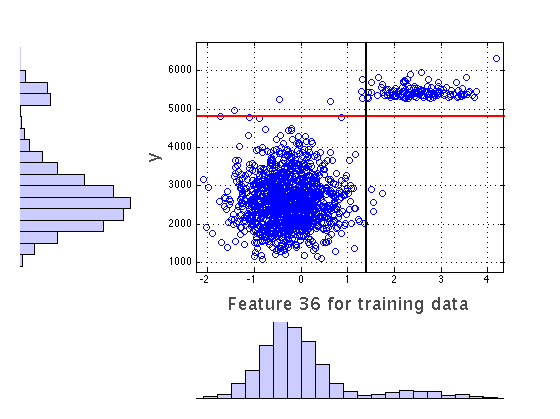
\includegraphics[width=2.5in]{figures/feature36.png} \label{fig:feature36}}
\hfill
\caption{}
\subfigure[Distribution of input variables.]{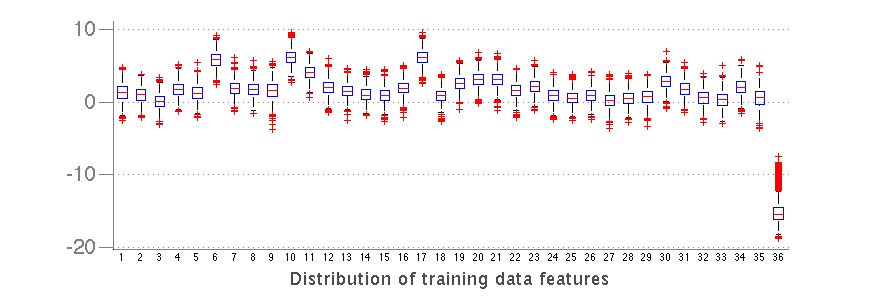
\includegraphics[width=2.5in]{figures/input_distribution_regression.png} \label{fig:regression_distribution}}
\hfill
\caption{}

begin{figure}
  begin{subfigure}[b]{0.4textwidth}
    includegraphics[width=textwidth]{figures/feature36.png}
    caption{Picture 1}
    label{fig:1}
  end{subfigure}
 
  begin{subfigure}[b]{0.4textwidth}
    includegraphics[width=textwidth]{figures/feature36.png}
    caption{Picture 2}
    label{fig:2}
  end{subfigure}
end{figure}

\end{figure}
We visually observed some linear correlations between certain features such as feature 2 and 24, 13 and 16, 17 and 20, but we decided to keep them since we did not have time to experiment with their removal or to test their signifance.
\textcolor{red}{TODO} We also removed some outliers using

\subsection{Baseline methods}
 We experimented with least squares using the normal equations, the least squares using gradient descent with alpha.  In both cases we obtained the same result. TODO talk about ill conditioned matriices.
 We report here our best results and parameters for every model. 
 For finding lambda we used 5 fold cross validation. We can see in figure [] the best results for this.
 The matrix was ill conditioned meaning some of the features were correlated, as expected also from our visualization. As Expected leastSquares gave NaN. We observed ridge regression did not improve much, we used a very small lambda. However, when we used polynomial features of degree 3,  with the same lambda and alpha, we obtained a significant improvement.
 
 Remove outliers for every feature. Plot the features also for the other regression
  
\section{Ridge regression}
We applied least-squares and ridge regression to this dataset. Since the matrix is ill-conditioned, least-squares is not suitable. Therefore, we report results obtained with ridge regression alone. Note that the improvements using ridge regression were modest and not much lower than that of linear regression, however we do not expect least-squares to work well when there is a lot of testing data available. 

Figure \ref{fig:ridgeCurve} shows the results obtained with ridge regression when we use $50\%$ of the data as test data and rest as training data. We varied the value of $\lambda$ from $10^{-4}$ to $10^3$, choosing total 500 points in between. We can see that there is a small improvement obtained for some values of $\lambda$.

We did experiments to plot a learning curve for this data (see Andrew Ng's notes about the learning curve). We held out 20\% of data as test data and rest as training data. We chose to slowly increase the proportion of data used for training. For each proportion of the training data, we repeated the experiment 30 times to compute the distribution of error. We fit ridge regression to each sampled training set and test it on the same $20\%$ test data. We varied the value of $\lambda$ from $10^{-4}$ to $10^3$, choosing total 500 points in between.

This gives us the learning curve shown in Fig. \ref{fig:learnCurve}. The blue curve shows the train error while red curve shows the test error. We can see that both training and test error converge, with the variance of estimates decreasing as we increase the training data size. There is also a very small gap between the train and test errors, showing that the linear model is a reasonable choice. The small gap exists perhaps because we have only limited test data.

\section{Feature transformations}
We tried several feature transformations. We found that we get a small improvement in performance when we take $\sqrt{|X_{ni}|}$ for all entries of $\mathbf{X}$. We did not check (due to lack of time) whether it matters if we apply this to one variable or all. We performed experiments similar to the last section (although one should really do cross-validation). Values of lambda were kept same as the last section. 

We compare three methods. First is a baseline where we do not use any input variables i.e. mean value of the output. The second method is the ridge regression described in previous section. The third method is ridge regression with a feature transformation. The first method gave RMSE of around 3 which was way worse than the other two methods.

The RMSE for the last two methods are shown in Fig. \ref{fig:summary}. We see that both test and train error decrease, however it appears that the improvement is very little and may not be significant.


\begin{figure}[!h]
\center
\subfigure[Ridge regression for a 50-50 split.]{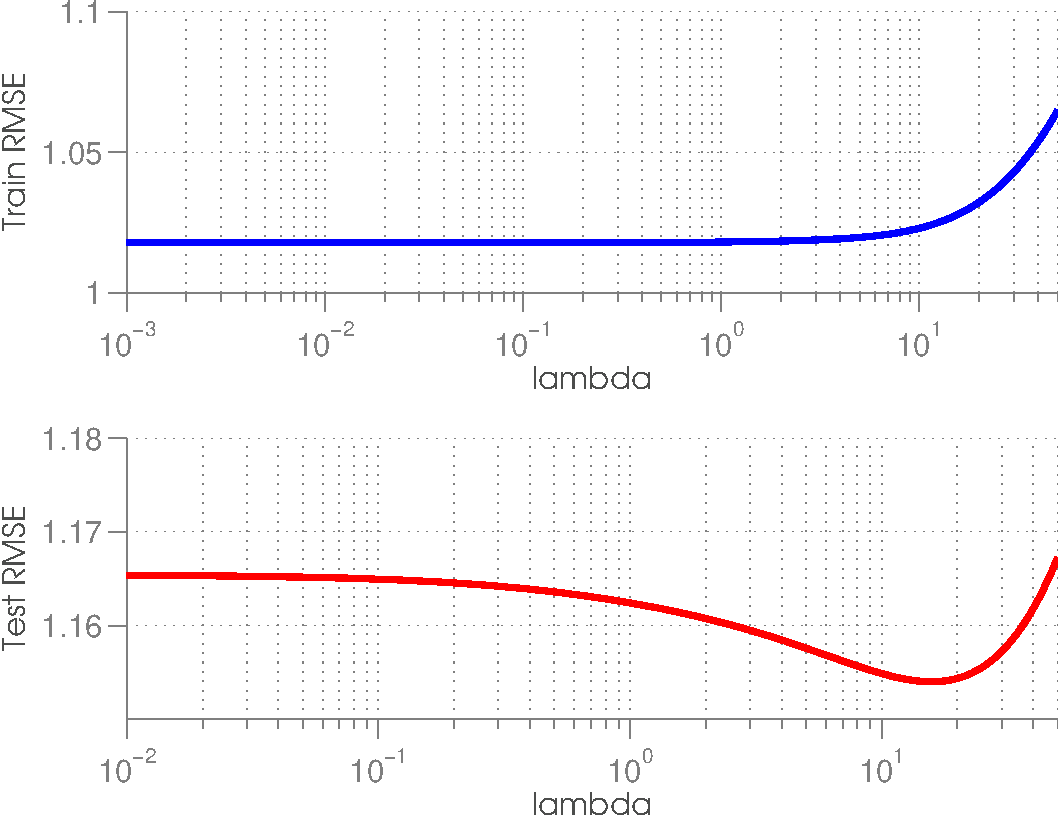
\includegraphics[width=2.5in]{figures/ridgeCurve.pdf} \label{fig:ridgeCurve}}
\hfill
\subfigure[Comparison of ridge regression with and without feature transformation. The improvement is very little and might be insignificant.]{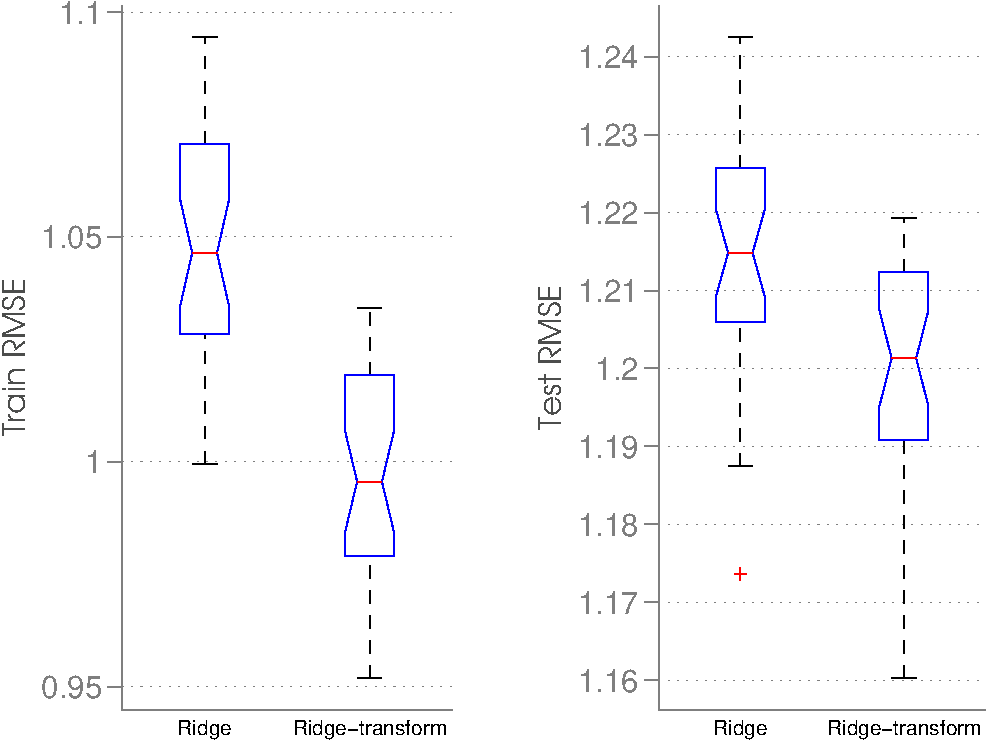
\includegraphics[width=2.7in]{figures/summary.pdf} \label{fig:summary}}
\subfigure[Learning curve. Blue is training data and red is test data.]{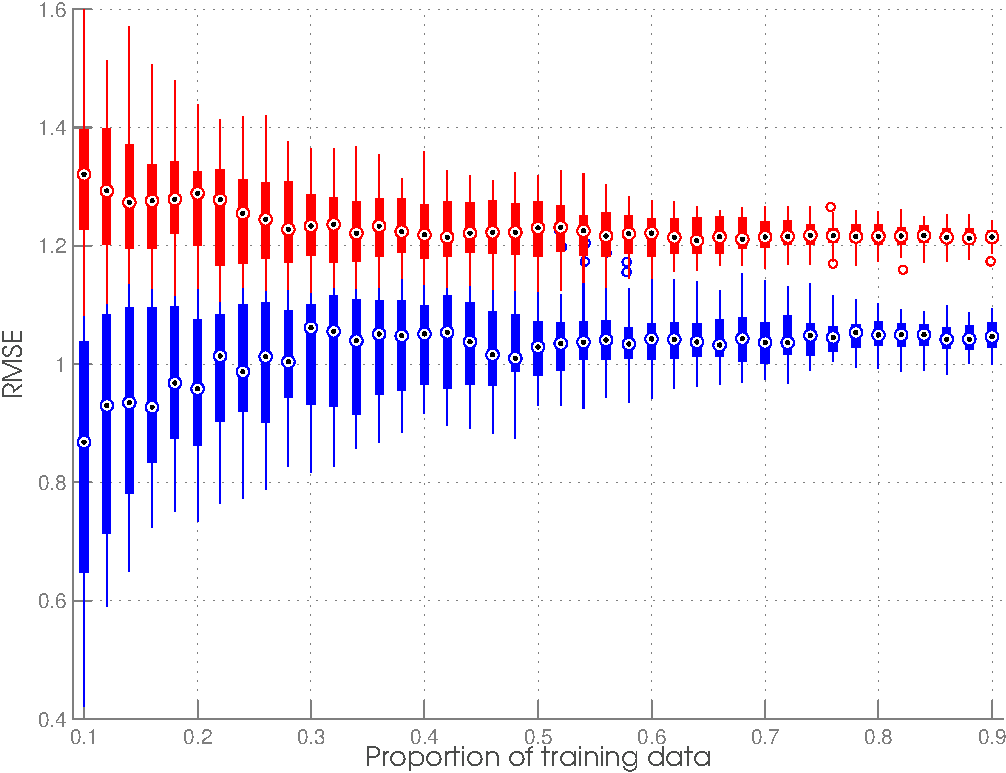
\includegraphics[width=4in]{figures/learningCurve.pdf} \label{fig:learnCurve}}
\caption{}
\end{figure}


\section{Summary}
In this report, we analyzed a regression dataset and found that ridge regression is a reasonable fit. We estimate that the average test error is 1.213 ($\pm$ 0.02). We tried some feature transformation and found that there is a small improvement giving us a test error of around 1.198 ($\pm$ 0.015). This improvement, however, is not significant.


\subsubsection*{Acknowledgments}
We would like to thank Timur for making the dataset for this study, Carlos and Ilija to help conduct the experiments, and all the students who attended the session making it exciting for us. All the code, as well as this report, was written by Emti. 

\subsubsection*{References}

\end{document}
